\documentclass{beamer}
\usetheme{Boadilla}
\useoutertheme[footline=authortitle]{}

\usepackage{verbatim} 
\usepackage{tikz} 
\usepackage{pgfgantt} 
\usepackage{ulem}
\usepackage{adjustbox} 

\usetikzlibrary{chains,shapes,arrows,calc}
\tikzstyle{line} = [draw, -latex']
\tikzstyle{box} = [rectangle, draw=black!50, align=left, font={\ttfamily}]
\tikzstyle{init} = [circle, draw=black!50]

\title{Higher Order Programming in Wybe}
\subtitle{MCS ``Work-In-Progress'' Presentation}
\author[James Barnes]
  {James Barnes (820946)}
\institute[unimelb]{University of Melbourne}
\date{Semester 2, 2021}

\begin{document}

\begin{frame}[plain, noframenumbering]
  \titlepage
  \vspace{-3.5em}
  \begin{center}
    \footnotesize Supervisor: Peter Schachte
  \end{center}
\end{frame}

\begin{frame}
  \frametitle{What is Wybe?}

  \begin{itemize}
    \item Looks \& feels imperative, yet programs declaratively
    \begin{itemize}
      \item Interface integrity
      \item Explicit data and control flow
    \end{itemize}
    \item Numerous novel language features
    \begin{itemize}
      \item Multiple inputs and outputs, with overloaded modes
      \item Resources
      \item Partial procedures (tests)
    \end{itemize}
    \item Novel intermediate representation, LPVM
    \begin{itemize}
      \item Currently lacks features present in other intermediate representations
    \end{itemize}
  \end{itemize}
\end{frame}

\begin{frame}[fragile]
  \frametitle{Wybe Features -- Overloaded Modes}

  \begin{itemize}
    \item Allows for procedures to be ``called in reverse''
  \end{itemize}
  \begin{example}[Overloaded modes]
    \begin{semiverbatim}
def add( x:int,  y:int, ?z:int) \{ ?z = x + y \}
def add( x:int, ?y:int,  z:int) \{ ?y = z - x \}
def add(?x:int,  y:int,  z:int) \{ ?x = z - y \}

?a = 1; ?b = 2
add(a, b, ?c)
\only<1>{add(a, ?d, c)}\only<2>{\sout{add(a, ?d, c)} \alert{?d = b}}
\end{semiverbatim}
\end{example}
\end{frame}

\begin{frame}[fragile]
  \frametitle{Wybe Features -- Resources}

  \begin{itemize}
    \item A by-name parameter-passing mechanism 
  \end{itemize}
  \begin{example}[Resource usage\only<2>{, flattened}]
    \begin{semiverbatim}
\uncover<1>{resource strings:list(string) = []}

def collect(tree:tree(string)\only<2>{, \alert{strings0, ?strings})})\only<1>{ use !strings} \{
    if \{ tree = node(?left, ?str, ?right) ::
          \uncover<1>!collect(left\only<2>{,  \alert{strings0, ?strings1}})
          \uncover<1>!collect(str\only<2>{,   \alert{strings1, ?strings2}}) 
          \uncover<1>!collect(right\only<2>{, \alert{strings2, ?strings}})
    \only<2>{   \alert{| else :: ?strings = strings0} }\}
\}

def collect(str:string\only<2>{, \alert{strings0, ?strings}})\only<1>{ use !strings} \{ 
    ?\alert<2>{strings} = \only<1>{strings }\only<2>{\alert{?strings0}} ,, [str] 
\}
\end{semiverbatim}
  \end{example}
\end{frame}

\begin{frame}
  \frametitle{Intermediate Representations \& LPVM}
  
  A compiler's representation of a program for analysis and transformation.

  \vspace{2em}

  Common intermediate representations each have their own problems:
  \begin{itemize}
    \item Name management problems, forward bias (impedes analyses)
  \end{itemize}
  
  Solutions?
  \begin{itemize}
    \item $\phi$-nodes, $\sigma$-nodes, $\gamma$-nodes, \dots 
    \item These are band-aids, only adding to the complexity
  \end{itemize}

  \vspace{2em}

  LPVM takes a paradigm shift into logic programming:
  \begin{itemize}
    \item Clauses are arranged such that non-determinism is tamed
  \end{itemize}
\end{frame}

\begin{frame}[fragile, noframenumbering, plain]
  \frametitle{LPVM vs SSA Form}

  \begin{columns}[t]
    \begin{column}{0.4 \textwidth}
      \centering
      Example:
    \end{column}
    \begin{column}{0.6 \textwidth}
      \centering
      SSA:
    \end{column}
  \end{columns}
  \begin{columns}
    \begin{column}{0.4 \textwidth}
      \centering
      {\small
      \begin{semiverbatim}
  int gcd(int a, int b) \{
      while (b != 0) \{
          int t = b;
          b = a \% t;
          a = t;
      \}
      return a;
  \}
\end{semiverbatim}}
    \end{column}
    \begin{column}{0.6 \textwidth}
      \centering
      \scalebox{0.75}{
        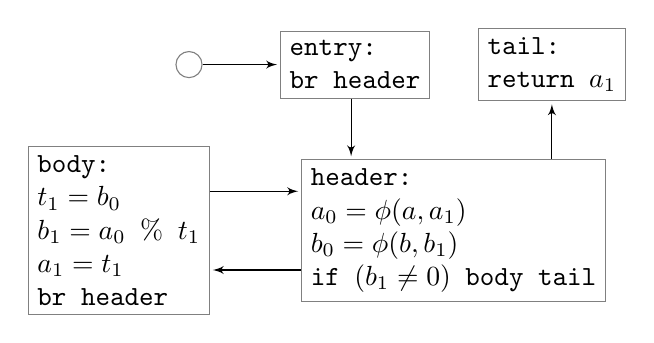
\begin{tikzpicture}[auto,
            shorten >=1pt, 
            node distance = 6em]
            \node [box] (header)    
              {header:\\
              $a_0 = \phi(a, a_1)$\\     
              $b_0 = \phi(b, b_1)$ \\
              if $(b_1 \neq 0)$ body tail};
            \node [box, above of=header] at (-1.25,0) (entry)    
              {entry:\\
              br header};      
            \node [init, left of=entry] (init) {};
            \node [box, above of=header] at (1.25,0) (tail)    
              {tail:\\
              return $a_1$};   
            \node [box] at (-4.25,0) (body)    
              {body:\\
            $t_1 = b_0$\\     
            $b_1 = a_0\ \%\ t_1$\\
            $a_1 = t_1$\\
            br header};
          \path [line] (init) -- (entry);
          \path [line] let \p0=($(entry.south)-(0.05,0)$), \p1=(header.north) in
            (\x0,\y0) -- (\x0,\y1);
          \path [line] let \p0=(tail.south), \p1=(header.north) in
            (\x0,\y1) -- (\x0,\y0);
          \path [line] ($(body.east)+(0,0.5)$) -- ($(header.west)+(0,0.5)$);
          \path [line] ($(header.west)-(0,0.5)$) -- ($(body.east)-(0,0.5)$);
        \end{tikzpicture}
      }
    \end{column}
  \end{columns}

  \vspace{2em}
  \begin{center}
    LPVM:
    \begin{equation*}
      \begin{array}{l}
        \mathtt{gcd(a, b, ?r) = b \neq 0\ \land\ mod(a, b, ?b^\prime)\ \land\ gcd(b, b^\prime, ?r)} \\
        \mathtt{gcd(a, b, ?r) = b = 0\,\ \land\,\ ?r = a}
      \end{array}
    \end{equation*}
  \end{center}     
\end{frame}


\begin{frame}
  \frametitle{What's Missing?}

  Higher order types! Unlike other language, Wybe does not support this feature.

  \vspace{2em}

  Higher order types allow you to\dots
  \begin{itemize}
    \item Write succinct and more general code
    \item Pass procedures into and out of other procedures
  \end{itemize}

  \vspace{2em}

  LPVM, which used by the Wybe compiler, also does not support higher order types.
\end{frame}

% \begin{frame}[fragile]
%   \frametitle{Higher Order Programming}

%   \footnotesize
%   \begin{example}[Higher order]
%     \begin{semiverbatim}
% map :: (a -> b) -> [a] -> [b]
% map f (a:as) = f a : map f as
% map f []     = []

% ls0 = map (+ 1)    [1,   2,   3  ]
% ls1 = map (* 3.14) [1.0, 2.0, 3.0]
% \end{semiverbatim}
%   \end{example}
  
%   \begin{example}[First order]
%     \begin{semiverbatim}
% mapPlus :: Int -> [Int] -> [Int]
% mapPlus x (a:as) = (a + x) : mapPlus x f as
% mapPlus x []     = []

% mapTimes :: Float -> [Float] -> [Float]
% mapTimes x (a:as) = (a * x) : mapTimes x f as
% mapTimes x []     = []

% ls0 = mapPlus  1    [1,   2,   3  ]
% ls1 = mapTimes 3.14 [1.0, 2.0, 3.0]
% \end{semiverbatim}
%   \end{example}
% \end{frame}

\begin{frame}
  \frametitle{Research \only<1>{Questions}\only<2>{\sout{Questions} \alert{Goals}}}

  \begin{enumerate}
    \item Can we \alert<2>{extend} the existing \alert<2>{Wybe features to support higher order types}?
    \item How can we \alert<2>{extend the LPVM implementation to support higher order types}?
    \item How does the existing Wybe implementation \alert<2>{compare} to \alert<2>{the extended Wybe type system in terms of performance}? 
  \end{enumerate}
\end{frame}

\begin{frame}
  \frametitle{Wybe Extension}

  We want to support higher order types in conjunction with the novel features of Wybe.

  \vspace{2em}

  \begin{itemize}
    \item Formalise, and extend, the Wybe type system to support higher order types
    \item Extending Wybe's features to support higher order types
    \begin{itemize}
      \item Multiple modes, resources
      \item Closures and anonymous functions
    \end{itemize}
    \item Parsing new syntax, etc.
  \end{itemize}
\end{frame}

\begin{frame}[fragile]
  \frametitle{Higher Order Wybe}

  \begin{example}[\only<1>{List operations}\only<2>{Fold implementation}]
    \begin{semiverbatim}
\only<1>{?list = [1, 2, 3, 4]

?sum = 0
for ?i in list \{
    ?sum = sum + i
\}
?prod = 1
for ?i in list \{
    ?prod = prod * i
\}

fold(\{ @ + @ = ?@ \}, 0, list, ?sum)
fold(\{ @ * @ = ?@ \}, 1, list, ?prod)}\only<2>{def fold(f:(:?a, :?b, ?:?b), b0:?b, as:list(?a), ?b:?b) \{
    ?b = b0
    for ?a in as \{
        f(a, b, ?b)
    \}
\}}
\end{semiverbatim}
  \end{example}
\end{frame}

\begin{frame}
  \frametitle{LPVM Extension}

  To support higher order types, the type system of LPVM must be extended.

  \vspace{2em}

  \begin{itemize}
    \item Formalisation of the existing LPVM type system
    \begin{itemize}
      \item Typing rules, and proofs, that specify valid typings in LPVM
    \end{itemize}
    \item Implementing higher order types within the formalised type system
    \item Various optimisations
  \end{itemize}
\end{frame}

\begin{frame}
  \frametitle{Performance Comparison}

  Ideally, higher order types should not cause major performance overheads.

  \vspace{2em}
  
  \begin{itemize}
    \item Creating higher order Wybe programs, transforming into first order
    \item Compare each compiled program pair
    \begin{itemize}
      \item Compare execution time \& code size
    \end{itemize}
  \end{itemize}

  \vspace{2em}

  Hypothesis: higher order code will cause a slowdown. 

  \vspace{1em}

  Hypothesis: programs may be more succinct, but require more code generation.
    
\end{frame}

\begin{frame}[fragile]
  \frametitle{Research Timeline}

  \centering
  \begin{adjustbox}{max totalsize={\textwidth}{.8\textheight},center}
    \begin{ganttchart}[
      x unit=0.45cm,
      y unit title=0.5cm,
      y unit chart=0.5cm,
      title height=1,
      vgrid, 
      hgrid,
    ]{1}{30}
      \gantttitle{2021 Sm2}{5}\gantttitle{Exam period/Break}{12}\gantttitle{2022 Sm1}{13}\\
      \ganttbar{Thesis writing}{15}{30} \\
      \ganttgroup{LPVM extension}{1}{8} \\
      \ganttgroup{Wybe extension}{9}{20} \\
      \ganttgroup{Evaluation}{21}{26} 
    \end{ganttchart}
  \end{adjustbox}
\end{frame}


\begin{frame}
  \frametitle{Thanks For Watching!}

  Any questions?
\end{frame}

% \begin{frame}[plain, noframenumbering, fragile]
%   \frametitle{Current Progress -- Syntax}

%   \begin{example}[Resourceful higher order syntax]
%     \begin{semiverbatim}
% def map(f:(:?a, ?:?b)\{!io\}, 
%         as:list(?a), ?bs:list(?b)) use !io \{
%     if \{ [?a | ?as] = as ::
%           !f(a, ?b)
%           !map(f, as, ?bs)
%           ?bs = [b | bs]
%        | otherwise :: 
%           ?bs = []
%        \}
% \}

% !map(\{ !read(?x); ?@2 = @1 * x \}, [1, 2, 3], ?bs)
% \# ...
% \end{semiverbatim}
%   \end{example}
% \end{frame}




\end{document}